2. $\cfrac{(x^2-8x+15)(x-5)(x^2-2x+3)}{(x^2-3x-18)(x+1)^2}\geqslant0\Leftrightarrow\cfrac{(x-3)(x-5)^2((x-1)^2+2)}{(x-6)(x+3)(x+1)^2}\geqslant0.$ Применив метод интервалов, найдём ответ: $x\in(-3;-1)\cup(-1;3]\cup\{5\}\cup(6;+\infty).$
\begin{figure}[ht!]
\center{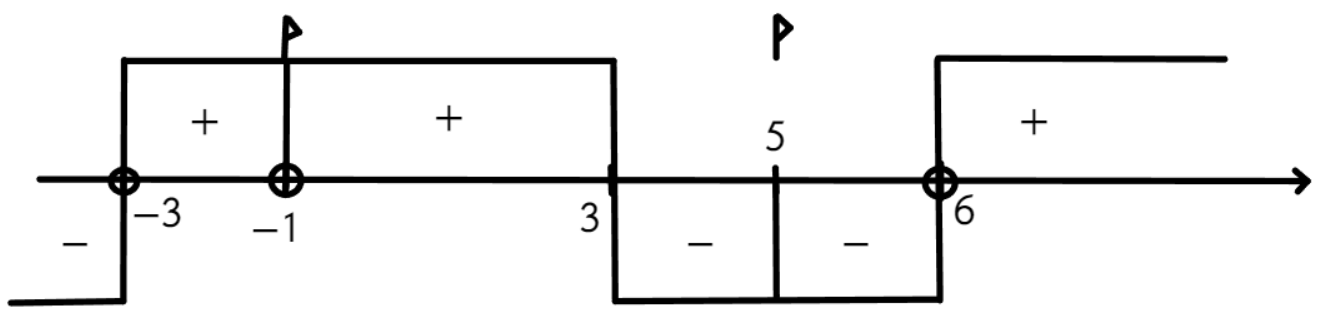
\includegraphics[scale=0.35]{ner9-2.png}}
\end{figure}\\
